\subsection{Output}
Output of the Xcos implementation is shown in the graphical window of scilab. One can also see the values using scilab code implementation. As the hand moves up-down, light intensity incident on LDR changes, and corresponding values being read by Arduino changes.
\begin{figure}
\centering
\includegraphics[width=\smfig]{\LocLDRfig/ldr_1.png}
\caption{Output}
\label{fig:ldrop-1}
\end{figure}


\begin{figure}
\centering
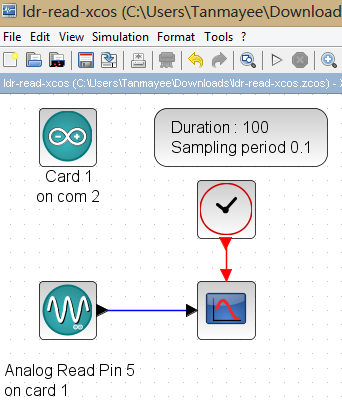
\includegraphics[width=\smfig]{\LocLDRfig/ldr-read-xcos.png}
\caption{Xcos diagram for LDR experiment}
\label{fig:ldrexpt-2}
\end{figure}

\subsection{Output}
Observe the value read by Arduino when high intensity is exposed. Value reaches to 1023. Below is the graphical window in Scilab which shows this value w.r.t 100 readings acquired iteratively using scilab-arduino toolbox. It is observed that value reaches 1023 when LDR is exposed to high intensity.
\begin{figure}
\centering
\includegraphics[width=\smfig]{\LocLDRfig/ldr_3.png}
\caption{Output}
\label{fig:ldrop-2}
\end{figure}

\section {Experiment: LED and LDR}


\subsection{Using Xcos diagram}
From the Arduino module Xcos following blocks will be used for the model:
\begin{figure}
\centering
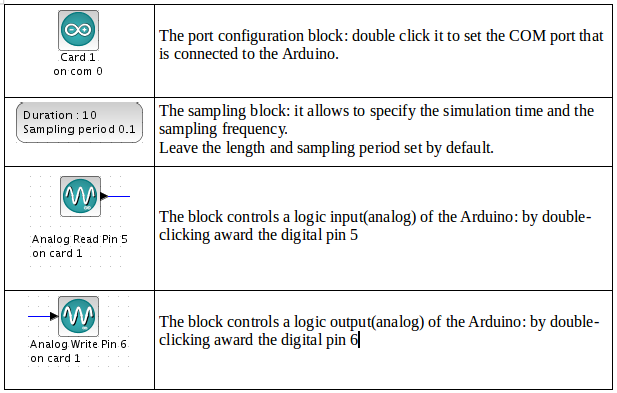
\includegraphics[width=\smfig]{\LocLDRfig/xcos_ldr.png}
\caption{Output}
\label{fig:xcosldrdesc-2}
\end{figure}

%\begin{figure}
%\centering
%\includegraphics[width=\smfig]{\LocLDRfig/ldr-sub-expt-3.png}
%\caption{Xcos diagram}
%\label{fig:xcosldr-3}
%\end{figure}

\subsection{Exercise}
\begin{enumerate}
\item Calculate the difference in LDR readings in indoor room before lighting the lamp and after lighting the lamp. You can also record changes in the room lighting at different times of the day.
\end{enumerate}

\section{Experiment: Interfacing temperature sensor using Scilab-Arduino toolbox}
This is the exercise where temperature sensor readings are acquired in scilab using arduino. Temperature sensor mounted on the shield is a thermistor. Operationally it performs similar to the LDR. Like in the case of LDR, its resistance varies as the temperature changes. This change in resistance can be transformed into change in voltage as in the case of LDR.

\begin{figure}
\centering
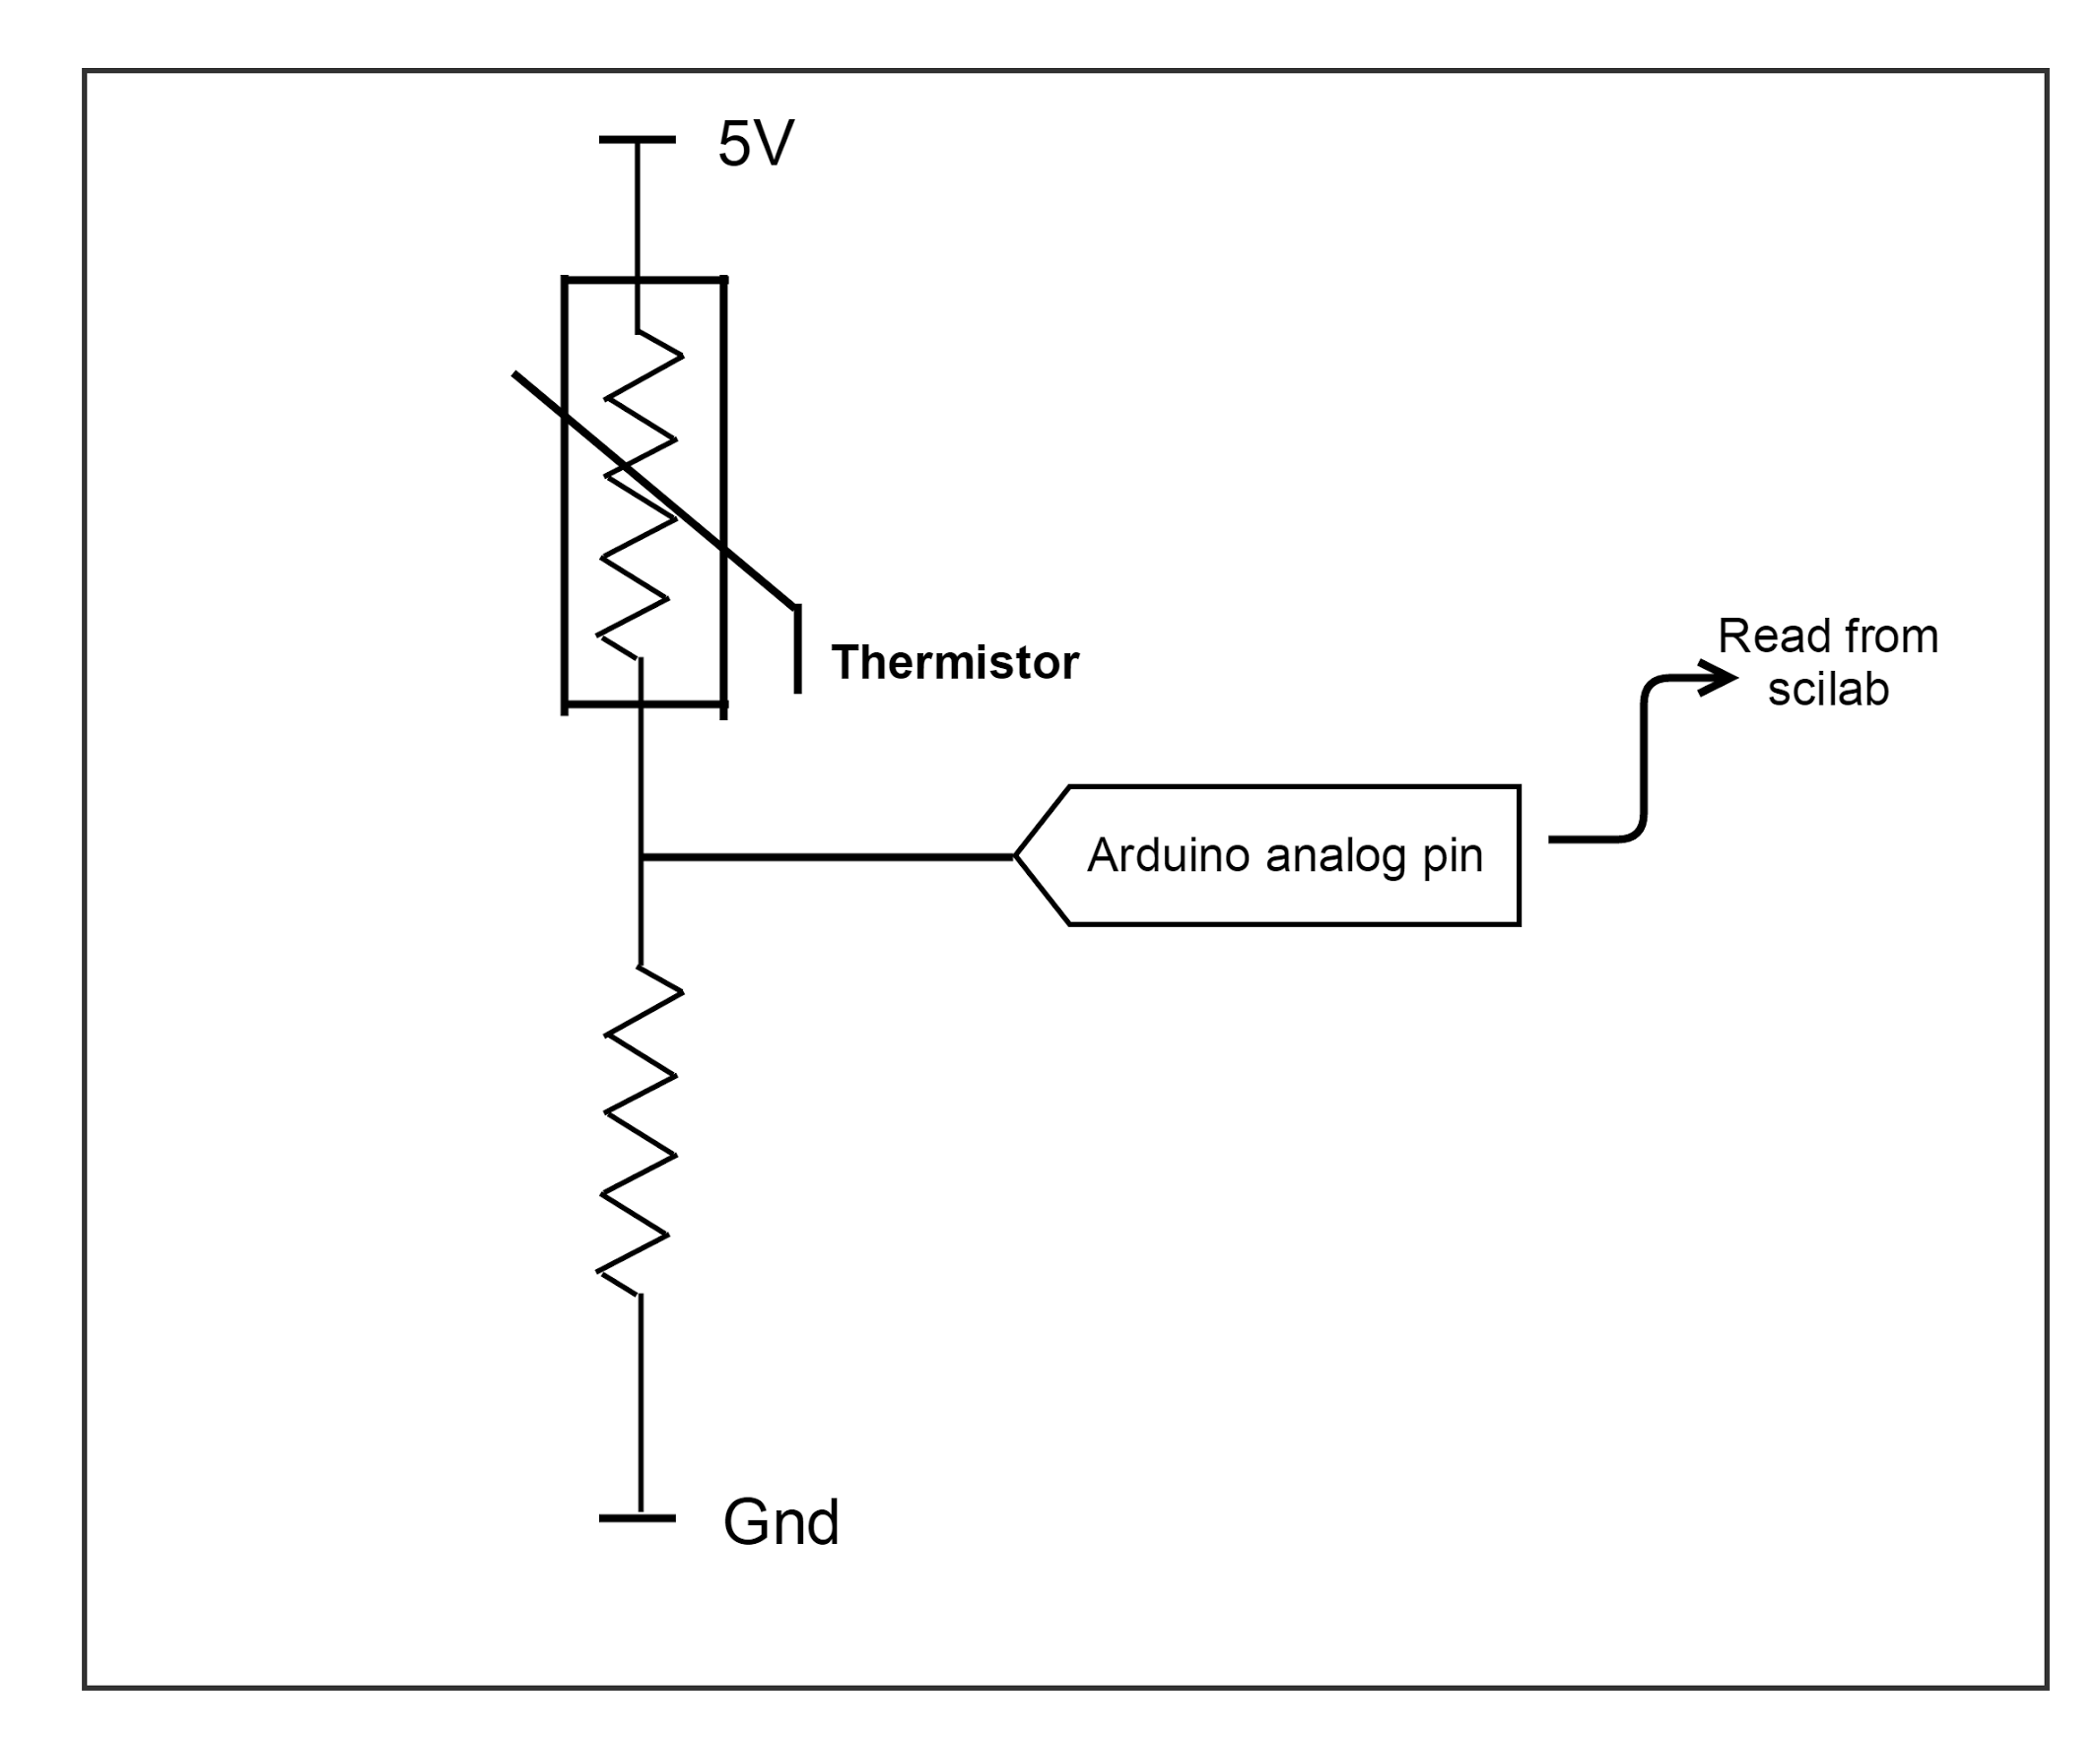
\includegraphics[width=\smfig]{\LocLDRfig/ldr-therm.png}
\caption{Connection diagram}
\label{fig:ldrtherm}
\end{figure}

\subsection{Connection}
As shown in the figure, temperature sensor is connected in series with resistor of known value  (10 k ohm in this case). Other terminals of resistor and thermistor are connected to  Gnd and Vcc respectively. Common terminal is given to analog input pin A4. 




\begin{figure}
\centering
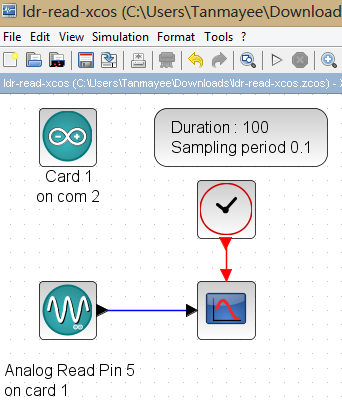
\includegraphics[width=\smfig]{\LocLDRfig/ldr-read-xcos.png}
\caption{Xcos Diagram to read LDR values}
\label{fig:xcos-ldr}
\end{figure}

%\begin{scicode}
%\ccaption{DC Motor Control}
%{DC Motor Control.  Available at
 % \LocLDRscibrief/dcmotor.sce.} 
%\label{sci:ldr-300}
%\lstinputlisting{\LocLDRscicode/dcmotor.sce}
%\end{scicode}




\subsection{Exercise}
User can perform same experiment as the sub-experiment 1 of LDR. By varying temperature near the thermistor using match stick/lighter, one can notice the change the values being read by arduino. Here we note that, arduino ADC hardware is being used to map analog voltage values into 0-1023 range. 
